\documentclass[12pt, letterpaper]{article}
\usepackage[utf8]{inputenc}
\usepackage{graphicx}
\usepackage{xcolor}
\usepackage{hyperref}
\definecolor{darkblue}{rgb}{0.0, 0.0, 0.55}
\hypersetup{
    colorlinks=true,
    linkcolor=darkblue,
    filecolor=darkblue,
    urlcolor=darkblue,
    citecolor=darkblue
}
\usepackage{amsmath}
\usepackage{booktabs}
\usepackage{caption}
\usepackage{geometry}
\usepackage{natbib}
\usepackage{tabularx}
\geometry{margin=1in}

\title{Stay, React, or Conform? Examining Social Influence Effects on Aesthetic Judgments}
\author{Omar Lizardo \& Sara Skiles}
\date{Revised Manuscript --- \today}

\begin{document}

\maketitle

\begin{abstract}
In this study, we address the question, foundational to sociological studies of taste, of the extent to which others' aesthetic judgments causally influence individual evaluations of cultural works, and how this influence depends on the social distance between self and other. While past research has documented observational associations between cultural tastes and social networks, the underlying causal mechanisms—whether individuals actively conform, react, or remain anchored in their initial judgments—have rarely been submitted to experimental test. Using a national survey experiment ($N = 2,275$), we manipulate exposure to peer aesthetic evaluations (likes vs.\ dislikes) and the status characteristics of the evaluating group across repeated trials. Using a difference-in-differences framework and inverse probability weighting, we find substantial evidence of \textit{valence asymmetry}: while negative peer evaluations broadly suppress positive exposure drift across groups, positive evaluations facilitate upward shifts conditionally based on status congruence. Furthermore, analyzing discrete behavioral choices shows that evaluative stability (``staying'') is not driven by high status alone, but by \textit{structural status consistency}: both high-consistent and low-consistent individuals display high evaluative inertia, whereas status-inconsistent individuals exhibit evaluative fluidity.
\end{abstract}

\newpage
\section{Introduction}

\subsection{Theoretical Background}
Taste expressions and consumption have long been shown to be a function of individuals' desire to differentiate themselves from others \citep{simmel1957, dimaggio1987}. \citet{bourdieu1984} suggests that taste differences evoke a visceral reaction, and it is through the rejection of others' aesthetic tastes that individuals engage in the symbolic boundary work that separates them. Thus, the expression of distastes serves to communicate social distance from certain social groups \citep{bryson1996, lamont2002}. In contexts where individuals discover a similarity in taste with members of a meaningful outgroup, they frequently engage in ``taste abandonment'' to maintain social boundaries \citep{berger2008}, while contexts in which individuals find a similarity of tastes with members of their ingroup can foster community and solidarity \citep{wohl2015community-2d2, vanzella2022tastes}.

Despite the rich sociological literature linking cultural tastes and network ties \citep{erickson1996, lizardo2006}, this body of work has almost exclusively relied on static, cross-sectional, and observational survey data. Consequently, observational homophily inevitably conflates prior social sorting, shared environmental exposure, and active social influence. This leaves open a fundamental causal question: \textit{How does direct access to the evaluations of others causally alter our own aesthetic judgments in real time?}

To answer this question, we build a theoretical framework that integrates three distinct mechanisms. First, in situations of aesthetic ambiguity, others' choices provide heuristic information to resolve uncertainty \citep{strang2001search-10a, salganik2006experimental-88d}. However, we expect a pronounced \textit{valence asymmetry}: negative peer evaluations act as a potent suppressive veto that halts the positive exposure drift observed under repeated evaluation, whereas positive peer evaluations act selectively depending on social status alignment.

Second, cultural influence is conditioned by the status of the evaluator relative to the self \citep{heider1946attitudes-ff3, bourdieu1984, lizardo2016cultural-aaa}. We examine whether individuals show same-status alignment, upward conformity to high-status cultural specialists, or reactive distancing from low-status evaluations.

Third, beyond linear mean shifts, individuals differ in their inertial propensity to maintain their initial judgment (``staying''). Drawing on status crystallization theory \citep{lenski1954status}, we propose that structural consistency between objective educational capital and subjective class identification produces cognitive certainty and evaluative inertia, whereas status inconsistency induces evaluative fluidity.

\subsection{Hypotheses}
Under the unexposed Control Condition, repeated exposure to a cultural object across trials is expected to produce an upward drift in evaluation even in the absence of external social information \citep{zajonc1968attitudinal, reber1998effects-efe}. External social cues either facilitate or suppress this exposure drift. In the case of generalized peer influence without status cues, exposure to positive peer evaluations is expected to facilitate this positive exposure drift, whereas exposure to negative peer evaluations exerts an asymmetric veto, suppressing the upward drift.

When status information is introduced, we test three hypotheses concerning intergroup dynamics. Under \textit{Hypothesis 1}, individuals adjust their judgments to align with the aggregate evaluations of their status peers, shifting positively for peer likes and negatively for peer dislikes. Under \textit{Hypothesis 2}, lower-status respondents align their judgments with high-status peers, exhibiting cultural goodwill toward high-status evaluations. Conversely, under \textit{Hypothesis 3}, individuals distance themselves from out-group judgments, shifting away from the evaluations of socially dissimilar others. Finally, regarding behavioral stability, under \textit{Hypothesis 4}, individuals with consistent status profiles (e.g., Middle Class with College, or Working Class without College) exhibit higher propensities to maintain their initial evaluation (``staying'') compared to status-inconsistent individuals.

\section{Data and Methods}

\subsection{Sample Recruitment and Survey Administration}
Data for this study were collected between February 28 and March 6, 2012, via an online experimental survey administered by Survey Sampling International (SSI), a leading research firm specializing in online panel recruitment and survey sampling. A total of 3,782 panel members accessed the survey instrument. Of these, 97 were excluded due to lack of informed consent ($N = 85$) or age under 18 ($N = 12$), 1,394 were screened out because demographic quota targets had already been met, and 16 dropped out during early screens, resulting in an analytic sample of $N = 2,275$ completed responses (with $N = 2,253$ providing complete initial and post-treatment evaluations). Participants received monetary compensation (\$3.92) via SSI, funded by an NSF Doctoral Dissertation Improvement Grant (Award SES-1203426) and the University of Notre Dame Institute for Scholarship in Liberal Arts.

The sampling frame employed dynamic quota matching calibrated against U.S. Census benchmarks for gender, age, race/ethnicity, and geographic region to achieve a diverse and quasi-representative national sample of U.S. adults. To ensure adequate statistical power for examining status-differentiated cultural dynamics—particularly within high-cultural-capital occupational cells (Cultural Specialists and Economic Specialists)—the sample incorporated a deliberate oversample of college graduates (40.5\% holding a bachelor's degree or higher in the sample versus approximately 28\% nationally in 2012). Table \ref{tbl:descriptives} presents the full demographic breakdown of the sample compared to U.S. population parameters, separated across experimental treatment arms.

\subsection{Inferential Scope and Interpretation of Confidence Intervals}
Because the survey used a quota-matched, opt-in online consumer panel rather than a strict probability-based sample with known inclusion probabilities (such as the GSS or ANES), the reported standard errors, $p$-values, and confidence intervals should be interpreted as reflecting \textit{model-based and experimental design uncertainty within the sample}, rather than formal design-based population parameter estimates. The randomization mechanism built into the Qualtrics survey engine ensures that internal validity is maximized: respondents were randomly assigned to treatment and control arms, creating balanced experimental groups across all observed baseline characteristics (Table \ref{tbl:descriptives}). At the same time, the demographic diversity across gender, age, race, and geographic region provides substantial ecological validity and heterogeneity compared to conventional undergraduate convenience samples.

\begin{table}[ht!]
\centering
\small
\caption{Demographic Characteristics of Survey Sample Compared to U.S. Population Benchmarks}
\label{tbl:descriptives}
\setlength{\tabcolsep}{4.5pt}
\begin{tabular*}{\linewidth}{@{\extracolsep{\fill}}lcccccc@{}}
\toprule
Demographic Variable & Sample $N$ & Sample \% & U.S. Pop \% & Treatment & No Alter & Taste Only \\
\midrule
\textbf{Gender} & & & & & & \\
\quad Women & 1,184 & 52.1\% & 51.5\% & 51.7\% & 52.2\% & 53.9\% \\
\quad Men & 1,091 & 47.9\% & 48.5\% & 48.3\% & 47.8\% & 46.1\% \\
\addlinespace[3pt]
\textbf{Race / Ethnicity} & & & & & & \\
\quad White & 1,463 & 64.3\% & 65.1\% & 64.7\% & 63.2\% & 63.1\% \\
\quad Hispanic / Latino & 365 & 16.1\% & 15.8\% & 16.2\% & 14.8\% & 15.9\% \\
\quad Black / African American & 279 & 12.3\% & 12.3\% & 12.1\% & 13.7\% & 12.1\% \\
\quad Asian / Pacific Islander & 103 & 4.5\% & 4.5\% & 4.4\% & 5.5\% & 4.6\% \\
\quad Other / Multiracial & 65 & 2.8\% & 2.3\% & 2.5\% & 2.7\% & 4.3\% \\
\addlinespace[3pt]
\textbf{Age Group} & & & & & & \\
\quad 18--24 & 272 & 12.0\% & 13.1\% & 11.9\% & 11.0\% & 12.7\% \\
\quad 25--34 & 410 & 18.0\% & 17.5\% & 18.2\% & 16.5\% & 17.9\% \\
\quad 35--44 & 402 & 17.7\% & 17.5\% & 17.9\% & 13.7\% & 18.7\% \\
\quad 45--54 & 441 & 19.4\% & 19.2\% & 19.4\% & 20.9\% & 18.4\% \\
\quad 55--64 & 372 & 16.3\% & 15.6\% & 16.5\% & 15.4\% & 16.1\% \\
\quad 65+ & 377 & 16.6\% & 17.2\% & 16.1\% & 22.5\% & 16.2\% \\
\addlinespace[3pt]
\textbf{Geographic Region} & & & & & & \\
\quad Northeast & 417 & 18.3\% & 17.9\% & 18.8\% & 16.5\% & 17.0\% \\
\quad South & 816 & 35.9\% & 37.2\% & 36.6\% & 39.6\% & 30.5\% \\
\quad Midwest & 505 & 22.2\% & 21.6\% & 21.2\% & 26.4\% & 24.8\% \\
\quad West & 536 & 23.6\% & 23.3\% & 23.4\% & 17.6\% & 27.7\% \\
\addlinespace[3pt]
\textbf{Education (Oversampled)} & & & & & & \\
\quad Less than High School & 89 & 3.9\% & 13.3\% & 3.8\% & 3.3\% & 4.6\% \\
\quad High School Diploma & 474 & 20.8\% & 30.4\% & 20.3\% & 23.6\% & 21.9\% \\
\quad Some College / AA & 791 & 34.8\% & 28.5\% & 36.0\% & 31.3\% & 30.6\% \\
\quad Bachelor's Degree & 625 & 27.5\% & 18.1\% & 27.3\% & 27.5\% & 28.5\% \\
\quad Graduate / Professional & 296 & 13.0\% & 9.6\% & 12.6\% & 14.3\% & 14.5\% \\
\midrule
\textbf{Total $N$} & \textbf{2,275} & \textbf{100.0\%} & & \textbf{1,746} & \textbf{182} & \textbf{347} \\
\bottomrule
\end{tabular*}
\begin{minipage}{\linewidth}
\vspace{4pt}
\footnotesize
\textit{Note:} U.S. population benchmarks are drawn from the 2010/2012 U.S. Census Bureau Current Population Survey (CPS). The analytic sample oversamples college-educated respondents to populate higher-status occupational cells.
\end{minipage}
\end{table}

\subsection{Experimental Design and Stimulus}
All respondents viewed an image of the same artwork: \textit{Nocturne: Blue and Gold -- Old Battersea Bridge} by James McNeill Whistler (1872), displayed in Figure \ref{fig:stimulus}. The painting was selected based on an online pilot study ($N=100$) testing eight artworks; the Whistler painting was chosen because it generated the highest initial pre-treatment variance in aesthetic evaluations across all demographic subgroups.

\begin{figure}[ht!]
    \centering
    
\includegraphics[width=0.55\textwidth]{figures/experimental_stimulus.jpeg}
    \caption{Experimental Stimulus: \textit{Nocturne: Blue and Gold -- Old Battersea Bridge}, by James McNeill Whistler (1872)}
    \label{fig:stimulus}
\end{figure}

The experiment used an incomplete factorial design with within-subject pre/post trials. In Trial 1, respondents provided their pre-treatment baseline rating of the painting on a 7-point Likert scale (1 = ``Dislike it very much'', 4 = ``Neither like nor dislike'', 7 = ``Like it very much''). Next, during an intervening survey block, respondents completed demographic questions and a musical taste battery before treatment respondents read a brief vignette describing how a peer group evaluated the artwork. Finally, in Trial 2, respondents were shown the painting again and provided their second evaluation.

To prevent terminological confusion, we strictly distinguish between the \textbf{pre-treatment baseline measurement} (Trial 1, which captures initial, uninfluenced aesthetic preference) and the \textbf{Control Condition} (the experimental group that receives no peer information between trials, allowing us to observe pure temporal re-evaluation in the absence of treatment). We refer to changes over repeated trials in this unexposed group as \textbf{exposure drift}.

To mitigate experimenter demand effects, the pre- and post-evaluations were separated by substantive survey modules, peer feedback was framed naturalistically as aggregate responses from a prior survey, and the no-information Control Condition was included to establish counterfactual re-evaluation dynamics.

\subsection{Variables and Measurement}
Aesthetic evaluation was measured on a reversed 1--7 scale. In continuous models, the outcome is the repeated evaluation across trials. In behavioral models, change between trials is categorized into three mutually exclusive choices: \textit{Stay} ($\Delta = 0$), \textit{Conform} (moving in the direction of the peer evaluation), and \textit{React} (moving in the opposite direction).

The treatment arms crossed peer evaluation (Like vs.\ Dislike) with peer social status. High-status peers were differentiated into Cultural Specialists (possessing multiple advanced degrees including a PhD and working in higher education) and Economic Specialists (holding a bachelor's degree in business and working in financial investment). Low-status peers were described as possessing a high school education and working in food service. In addition, two Taste-Only conditions provided peer like or dislike evaluations without any status indicators, and a pure Control Condition provided no peer information between trials ($N=182$).

We crossed objective education (College Degree vs.\ No College) with subjective class identification (Middle Class vs.\ Working Class) into four quadrants: Working/No College, Working/College, Middle/No College, and Middle/College.

A key methodological challenge in experimental designs that examine status-contingent influence arises from the hybrid nature of the design. While the experimental cues (peer evaluation valence and peer status) were randomly assigned, respondents' own social locations—captured by the crossing of educational attainment and subjective class identification—represent pre-existing, observational attributes \citep{cruces2013biases}. Consequently, individuals do not have an equal probability of belonging to each status group: for example, Middle Class individuals with a college degree are systematically older, more likely to have college-educated parents, and differ in racial/ethnic composition compared to non-college Working Class individuals. If unaddressed, comparisons across status groups (and their interactions with the randomized peer treatments) risk confounding the effect of social class with these correlated background characteristics.

To solve this problem and strengthen causal inference, we implement Inverse Probability Weighting (IPW) using generalized propensity scores \citep{rosenbaum1983central}. The logic of IPW proceeds in two steps. First, for each respondent, we estimate a multinomial logistic regression modeling the probability of belonging to their observed status consistency group $S_i \in \{1, 2, 3, 4\}$ conditional on exogenous baseline covariates $\mathbf{X}_i$ (age, gender, race/ethnicity, and parental educational capital): $e_s(\mathbf{X}_i) = P(S_i = s \mid \mathbf{X}_i)$. Second, each observation is weighted by the inverse of its estimated propensity score to target the Average Treatment Effect (ATE) across the pooled sample: $w_i = 1 / e_s(\mathbf{X}_i) = 1 / P(S_i = s \mid \mathbf{X}_i)$.

Intuitively, IPW creates a synthetic ``pseudo-population'' by up-weighting underrepresented demographic profiles within each status group (e.g., working-class respondents whose parents completed college) and down-weighting overrepresented profiles. This weighting scheme breaks the empirical association between the baseline covariates $\mathbf{X}_i$ and status group membership. Under the assumption of conditional exchangeability (no unmeasured confounders given $\mathbf{X}_i$) and positivity, IPW ensures that status groups are demographically comparable. As a result, subsequent differences in evaluative shifts, behavioral inertia, or reactance across status categories can be interpreted as the direct consequence of structural status location and status consistency, rather than demographic artifacts.

\subsection{Difference-in-Differences Analytic Strategy}
To strictly isolate information-induced shifts from repeated-measurement exposure drift, we formulate our analysis within a Difference-in-Differences (DiD) framework. Rather than examining simple pre-to-post changes within each condition in isolation—which conflates the effect of peer information with the natural exposure drift that occurs upon viewing an artwork a second time—the DiD strategy compares every treatment condition against the unexposed Control Condition.

Accordingly, we specify a linear mixed-effects model with random intercepts for respondents of the form:

\begin{equation}
\begin{split}
\text{Taste}_{ijt} = {} & \beta_0 + \beta_{1} \text{Trial}_{it} + \sum_{k=2}^{K} \beta_{k} \text{Cond}_{ik} \\
                        & + \sum_{k=1}^{K} \delta_{k} (\text{Trial}_{it} \times \text{Cond}_{ik}) + \mathbf{X}_i \boldsymbol{\gamma} + u_i + \epsilon_{ijt}
\end{split}
\label{eq:did_model}
\end{equation}

Where $i$ indexes individual respondents, $j$ indexes observations, $t \in \{1, 2\}$ indexes trials, and the unexposed Control Condition serves as the omitted reference category for the experimental condition effect $\text{Cond}_{ik}$.

The intercept ($\beta_0$) represents the expected baseline aesthetic evaluation at Trial 1 (pre-treatment) for respondents assigned to the unexposed Control Condition: $\beta_0 = E[\text{Taste} \mid \text{Trial} = 1, \text{Control}]$. The Trial main effect ($\beta_{1}$) captures the counterfactual \textit{exposure drift} from Trial 1 to Trial 2 in the absence of external peer information: $\beta_{1} = E[\text{Taste} \mid \text{Trial} = 2, \text{Control}] - E[\text{Taste} \mid \text{Trial} = 1, \text{Control}]$. When repeated viewing induces an intrinsic appreciation of the artwork (the mere exposure effect), $\beta_{1}$ should be positive and statistically significant.

The condition main effects ($\beta_k$) reflect pre-treatment differences between condition $k$ and the Control Condition at Trial 1: $\beta_k = E[\text{Taste} \mid \text{Trial} = 1, \text{Cond} = k] - E[\text{Taste} \mid \text{Trial} = 1, \text{Control}]$. Because respondents were randomly assigned to experimental conditions before viewing the painting, these coefficients assess baseline balance and are expected to be close to zero. The interaction coefficients ($\delta_k$) represent the \textit{causal Difference-in-Differences treatment effects}. Each $\delta_k$ measures whether the change in evaluations from Trial 1 to Trial 2 in treatment condition $k$ differed significantly from the change observed in the unexposed Control Condition:

\begin{equation}
\begin{split}
\delta_k = {} & \left( E[\text{Taste} \mid \text{Trial} = 2, k] - E[\text{Taste} \mid \text{Trial} = 1, k] \right) \\
              & - \left( E[\text{Taste} \mid \text{Trial} = 2, \text{Control}] - E[\text{Taste} \mid \text{Trial} = 1, \text{Control}] \right)
\end{split}
\end{equation}

Substantively, $\delta_k$ directly answers the counterfactual question: \textit{Did exposure to peer evaluation $k$ cause respondents' aesthetic judgments to change significantly more or less than they would have changed under mere repeated exposure alone?} A positive estimate ($\delta_k > 0$) indicates that peer feedback facilitated aesthetic appreciation beyond natural exposure drift, whereas a negative estimate ($\delta_k < 0$) indicates that peer feedback suppressed or reversed the positive exposure drift that would have naturally occurred.\footnote{
By the Frisch-Waugh-Lovell theorem, estimating Equation \ref{eq:did_model} via linear mixed models with individual random intercepts ($u_i$) is mathematically equivalent to regressing individual change scores ($\Delta \text{Taste}_i = \text{Taste}_{i2} - \text{Taste}_{i1}$) on the treatment indicators with the Control Condition as the omitted reference group:
\begin{equation}
\Delta \text{Taste}_i = \beta_{\text{Trial}} + \sum_{k=1}^{K} \delta_k \text{Cond}_{ik} + \epsilon_i
\end{equation}
where the intercept directly estimates the control exposure drift ($\beta_{1}$) and the condition slopes estimate the DiD treatment effects ($\delta_k$).} To examine non-linear behavioral choices, we also estimate multinomial logistic regressions modeling the discrete probabilities of Staying, Conforming, and Reacting.

\section{Results}

\subsection{Covariate Balance Across Observational Status Categories}
Before evaluating our focal hypotheses, we assessed the demographic comparability of the four observational status consistency groups. It is important to emphasize that while the experimental conditions (peer liking vs.\ disliking and peer status cues) were randomized and thus inherently balanced by design, respondents' own structural locations (Education $\times$ Subjective Class) are observational. 

Figure \ref{fig:balance} displays the standardized mean differences (SMD) for all baseline covariates across the status categories before and after Inverse Probability Weighting (IPW), generated using \texttt{cobalt} \citep{greifer2022cobalt}. Prior to weighting, status groups exhibited substantial demographic disparities: for instance, college-educated middle-class respondents had older ages and higher rates of parental college attainment (raw SMDs exceeding 0.35 to 0.50). Following IPW estimation, the weighted pseudo-population achieved balance, with all absolute standardized mean differences compressed well below the conventional conservative threshold of 0.10 standard deviations. This confirms that subsequent model estimates isolate the effect of social class and status consistency, net of observed demographic sorting.

\begin{figure}[ht!]
    \centering
    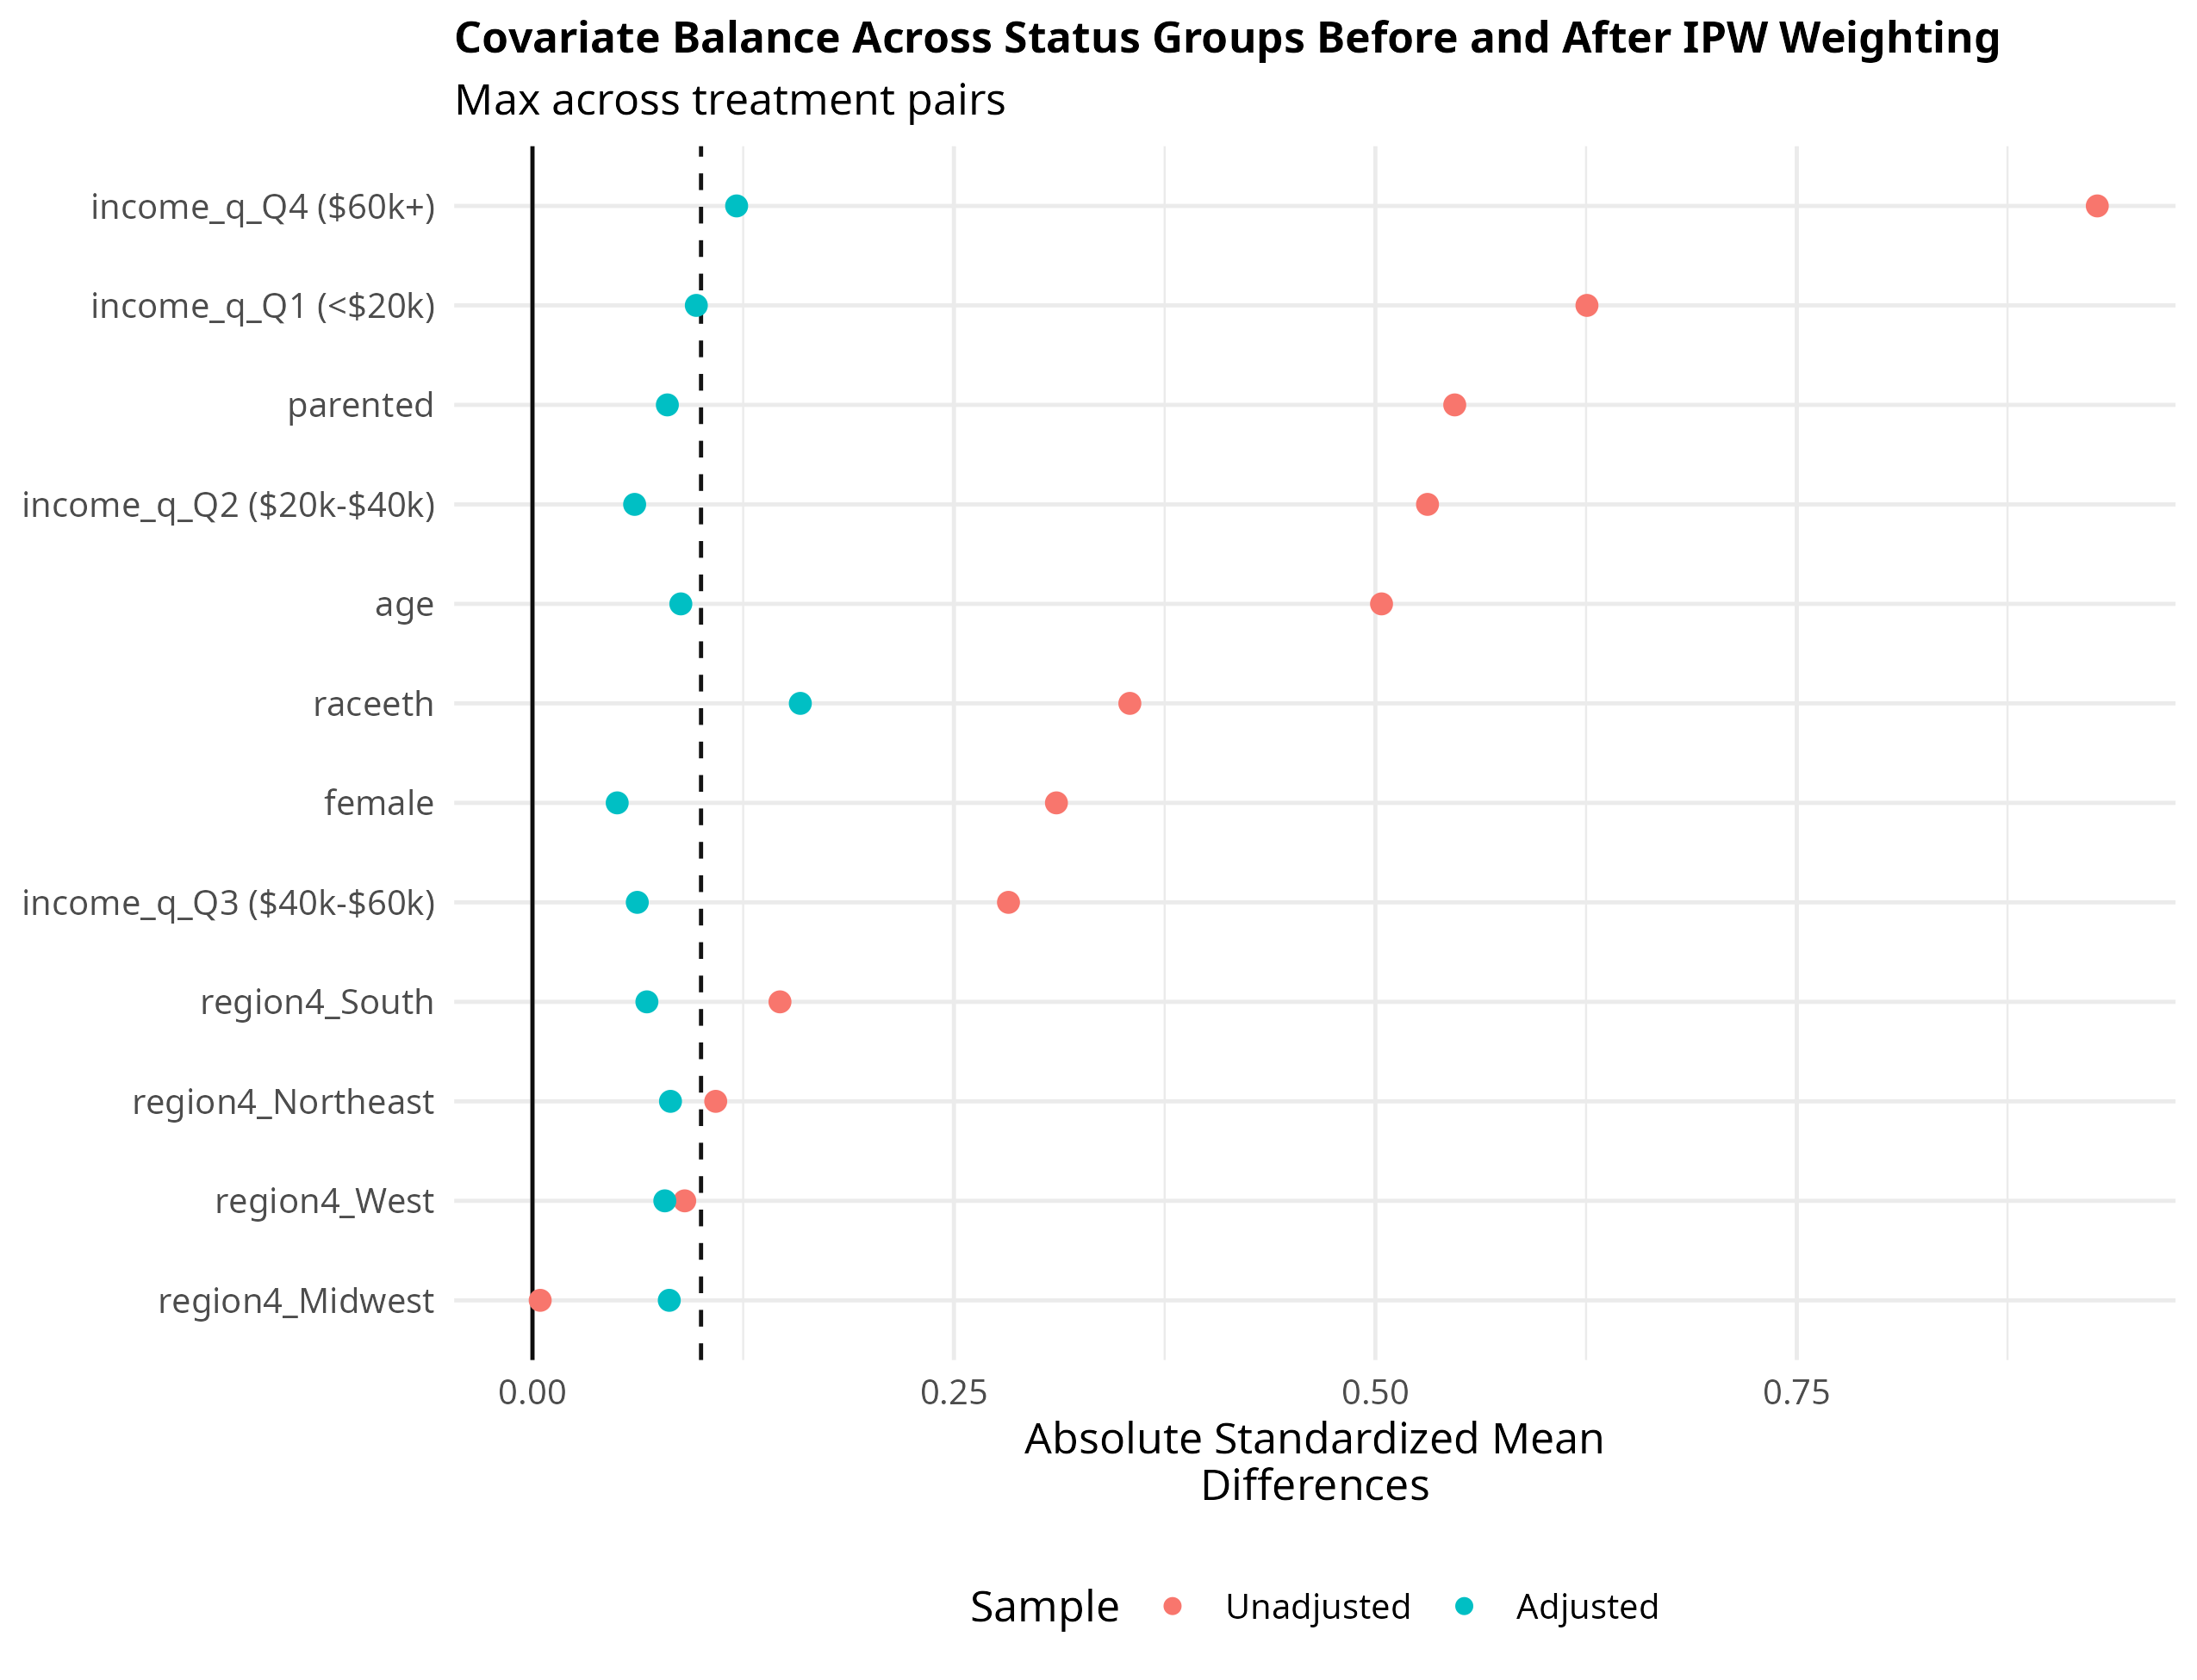
\includegraphics[width=0.8\textwidth]{figures/Figure8_CovariateBalance.png}
    \caption{Covariate Balance Across Observational Status Groups Before and After IPW Weighting. The dashed lines indicate the standard $\pm 0.10$ threshold for acceptable balance.}
    \label{fig:balance}
\end{figure}

\subsection{Counterfactual Exposure Drift in the Control Condition}
Evaluating the unexposed Control Condition allows us to observe the counterfactual drift in aesthetic judgments over repeated trials in the complete absence of peer cues. As shown in Table \ref{tbl:did_models}, repeated evaluation alone produces an upward drift in aesthetic liking ($\beta_{\text{Trial}} = +0.107, p = 0.041$ unweighted; $\beta_{\text{Trial}} = +0.156, p = 0.0038$ IPW-weighted).

Importantly, disaggregating by educational capital reveals that this exposure drift is not uniform. For respondents without a college degree, the counterfactual drift is zero ($\beta_{\text{Trial}} = 0.000, p = 1.00$). In contrast, college-educated respondents exhibit a substantial positive exposure drift ($\beta_{\text{Trial}} = +0.257, p = 0.016$). Thus, the mere exposure effect is conditioned by educational capital: individuals with higher cultural capital experience an intrinsic appreciation upon re-evaluation, whereas non-college individuals do not.

\subsection{Valence Asymmetry in Difference-in-Differences Effects}
Table \ref{tbl:did_models} and Figure \ref{fig:did_pooled} present the Difference-in-Differences (DiD) estimates comparing each treatment condition against the unexposed Control Condition.

\begin{table}[ht!]
\centering
\small
\caption{Difference-in-Differences (DiD) Linear Mixed Models Predicting Aesthetic Evaluation}
\label{tbl:did_models}
\setlength{\tabcolsep}{4.5pt}
\begin{tabular*}{\linewidth}{@{\extracolsep{\fill}}lcccc@{}}
\toprule
 & \multicolumn{2}{c}{\textbf{Model 1: Unweighted DiD}} & \multicolumn{2}{c}{\textbf{Model 2: IPW-Weighted DiD}} \\
\cmidrule(lr){2-3} \cmidrule(lr){4-5}
\textbf{Independent Variable} & Estimate (SE) & $t$ value & Estimate (SE) & $t$ value \\
\midrule
Intercept ($\beta_0$) & 4.689 (0.114) & 40.99$^{***}$ & 4.672 (0.115) & 40.72$^{***}$ \\
Trial 2 Exposure Drift ($\beta_{\text{Trial}}$) & 0.107 (0.052) & 2.05$^{*}$ & 0.156 (0.054) & 2.90$^{**}$ \\
\addlinespace[3pt]
\multicolumn{5}{l}{\textit{Difference-in-Differences Treatment Effects ($\text{Trial} \times \text{Condition}$):}} \\
Class \& Taste / Like / $-$Status & $-0.128$ (0.067) & $-1.93^{\dagger}$ & $-0.112$ (0.069) & $-1.61$ \\
Class \& Taste / Like / $+$Status & $+0.041$ (0.060) & 0.68 & $+0.006$ (0.062) & 0.09 \\
Class \& Taste / Dislike / $-$Status & $+0.016$ (0.066) & 0.23 & $-0.034$ (0.068) & $-0.49$ \\
Class \& Taste / Dislike / $+$Status & $-0.121$ (0.060) & $-2.02^{*}$ & $-0.201$ (0.062) & $-3.27^{**}$ \\
Taste Only / Like & $+0.096$ (0.075) & 1.29 & $+0.068$ (0.078) & 0.87 \\
Taste Only / Dislike & $-0.125$ (0.075) & $-1.67^{\dagger}$ & $-0.172$ (0.076) & $-2.26^{*}$ \\
\addlinespace[3pt]
Condition Main Effects Included & \multicolumn{2}{c}{Yes} & \multicolumn{2}{c}{Yes} \\
Random Intercept Variance ($\sigma^2_u$) & \multicolumn{2}{c}{2.074} & \multicolumn{2}{c}{2.026} \\
Residual Variance ($\sigma^2_e$) & \multicolumn{2}{c}{0.243} & \multicolumn{2}{c}{1.022} \\
$N$ (Observations / Individuals) & \multicolumn{2}{c}{4,506 / 2,253} & \multicolumn{2}{c}{4,504 / 2,252} \\
\bottomrule
\end{tabular*}
\begin{minipage}{\linewidth}
\vspace{4pt}
\footnotesize
\textit{Note:} $^{\dagger}p < 0.10, ^{*}p < 0.05, ^{**}p < 0.01, ^{***}p < 0.001$. Estimates represent Difference-in-Differences interactions relative to the unexposed Control Condition. Model 2 incorporates Inverse Probability Weighting (IPW) on age, gender, race/ethnicity, and parental education.
\end{minipage}
\end{table}

\begin{figure}[ht!]
    \centering
    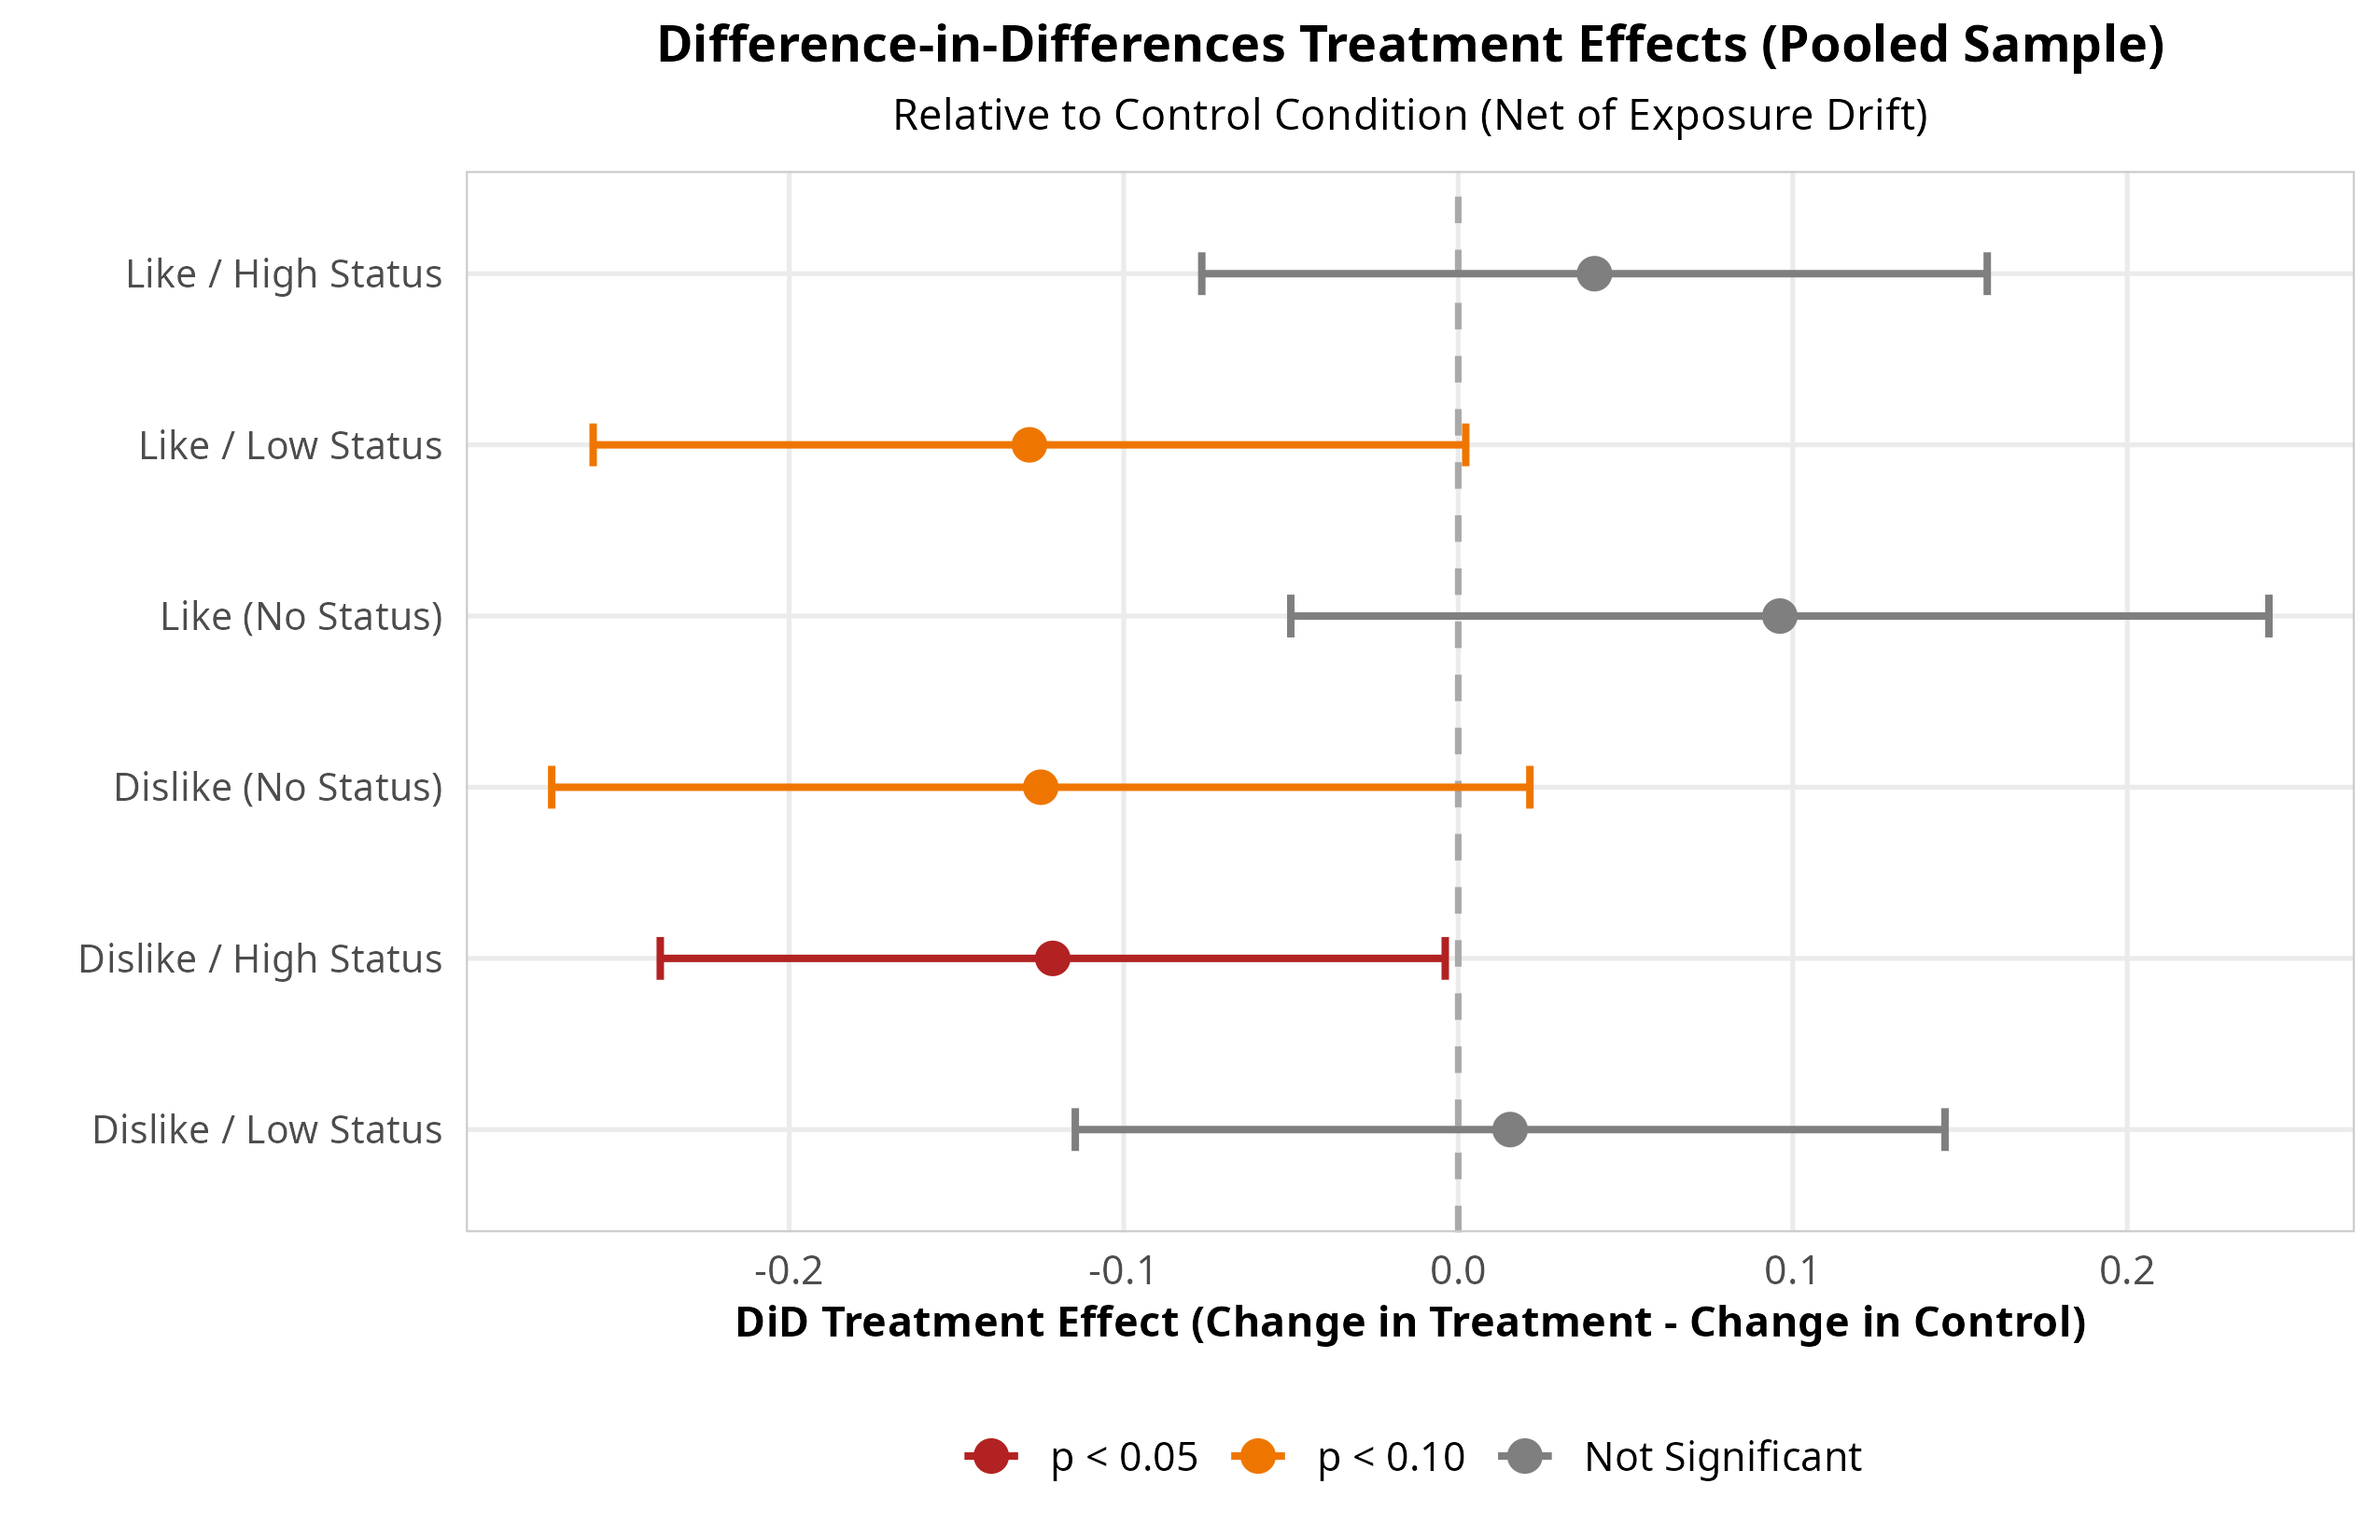
\includegraphics[width=0.85\textwidth]{figures/Figure_DiD_Forest_Pooled.png}
    \caption{Causal Difference-in-Differences Treatment Effects (Pooled Sample). Points represent point estimates and error bars denote 95\% confidence intervals net of control exposure drift.}
    \label{fig:did_pooled}
\end{figure}

The DiD results show clear evidence of valence asymmetry through two contrasting patterns. First, negative feedback acts as a suppresive. In the pooled sample, negative evaluations significantly halt and reverse the positive exposure drift. Exposure to High-Status Dislike leads to a significant negative divergence of $\text{DiD} = -0.201$ ($SE = 0.062, t = -3.27, p = 0.0011$) relative to the control condition. Generalized Dislike (Taste Only) similarly exerts a significant suppressive DiD effect of $\text{DiD} = -0.172$ ($SE = 0.076, t = -2.26, p = 0.0238$).

Second, positive peer feedback produces selective facilitation. Exposure to positive peer evaluations yields modest positive increments above the exposure drift ($\text{DiD} = +0.068$ to $+0.096$, $p > 0.15$). Thus, while cultural ``likes'' facilitate upward movement, negative peer evaluations act as a veto that halts natural aesthetic appreciation across the board.

\subsection{Status-Differentiated Influence: Testing Hypotheses 1--3}
Figure \ref{fig:did_status} displays the Difference-in-Differences treatment effects disaggregated across the four status consistency groups.

\begin{figure}[ht!]
    \centering
    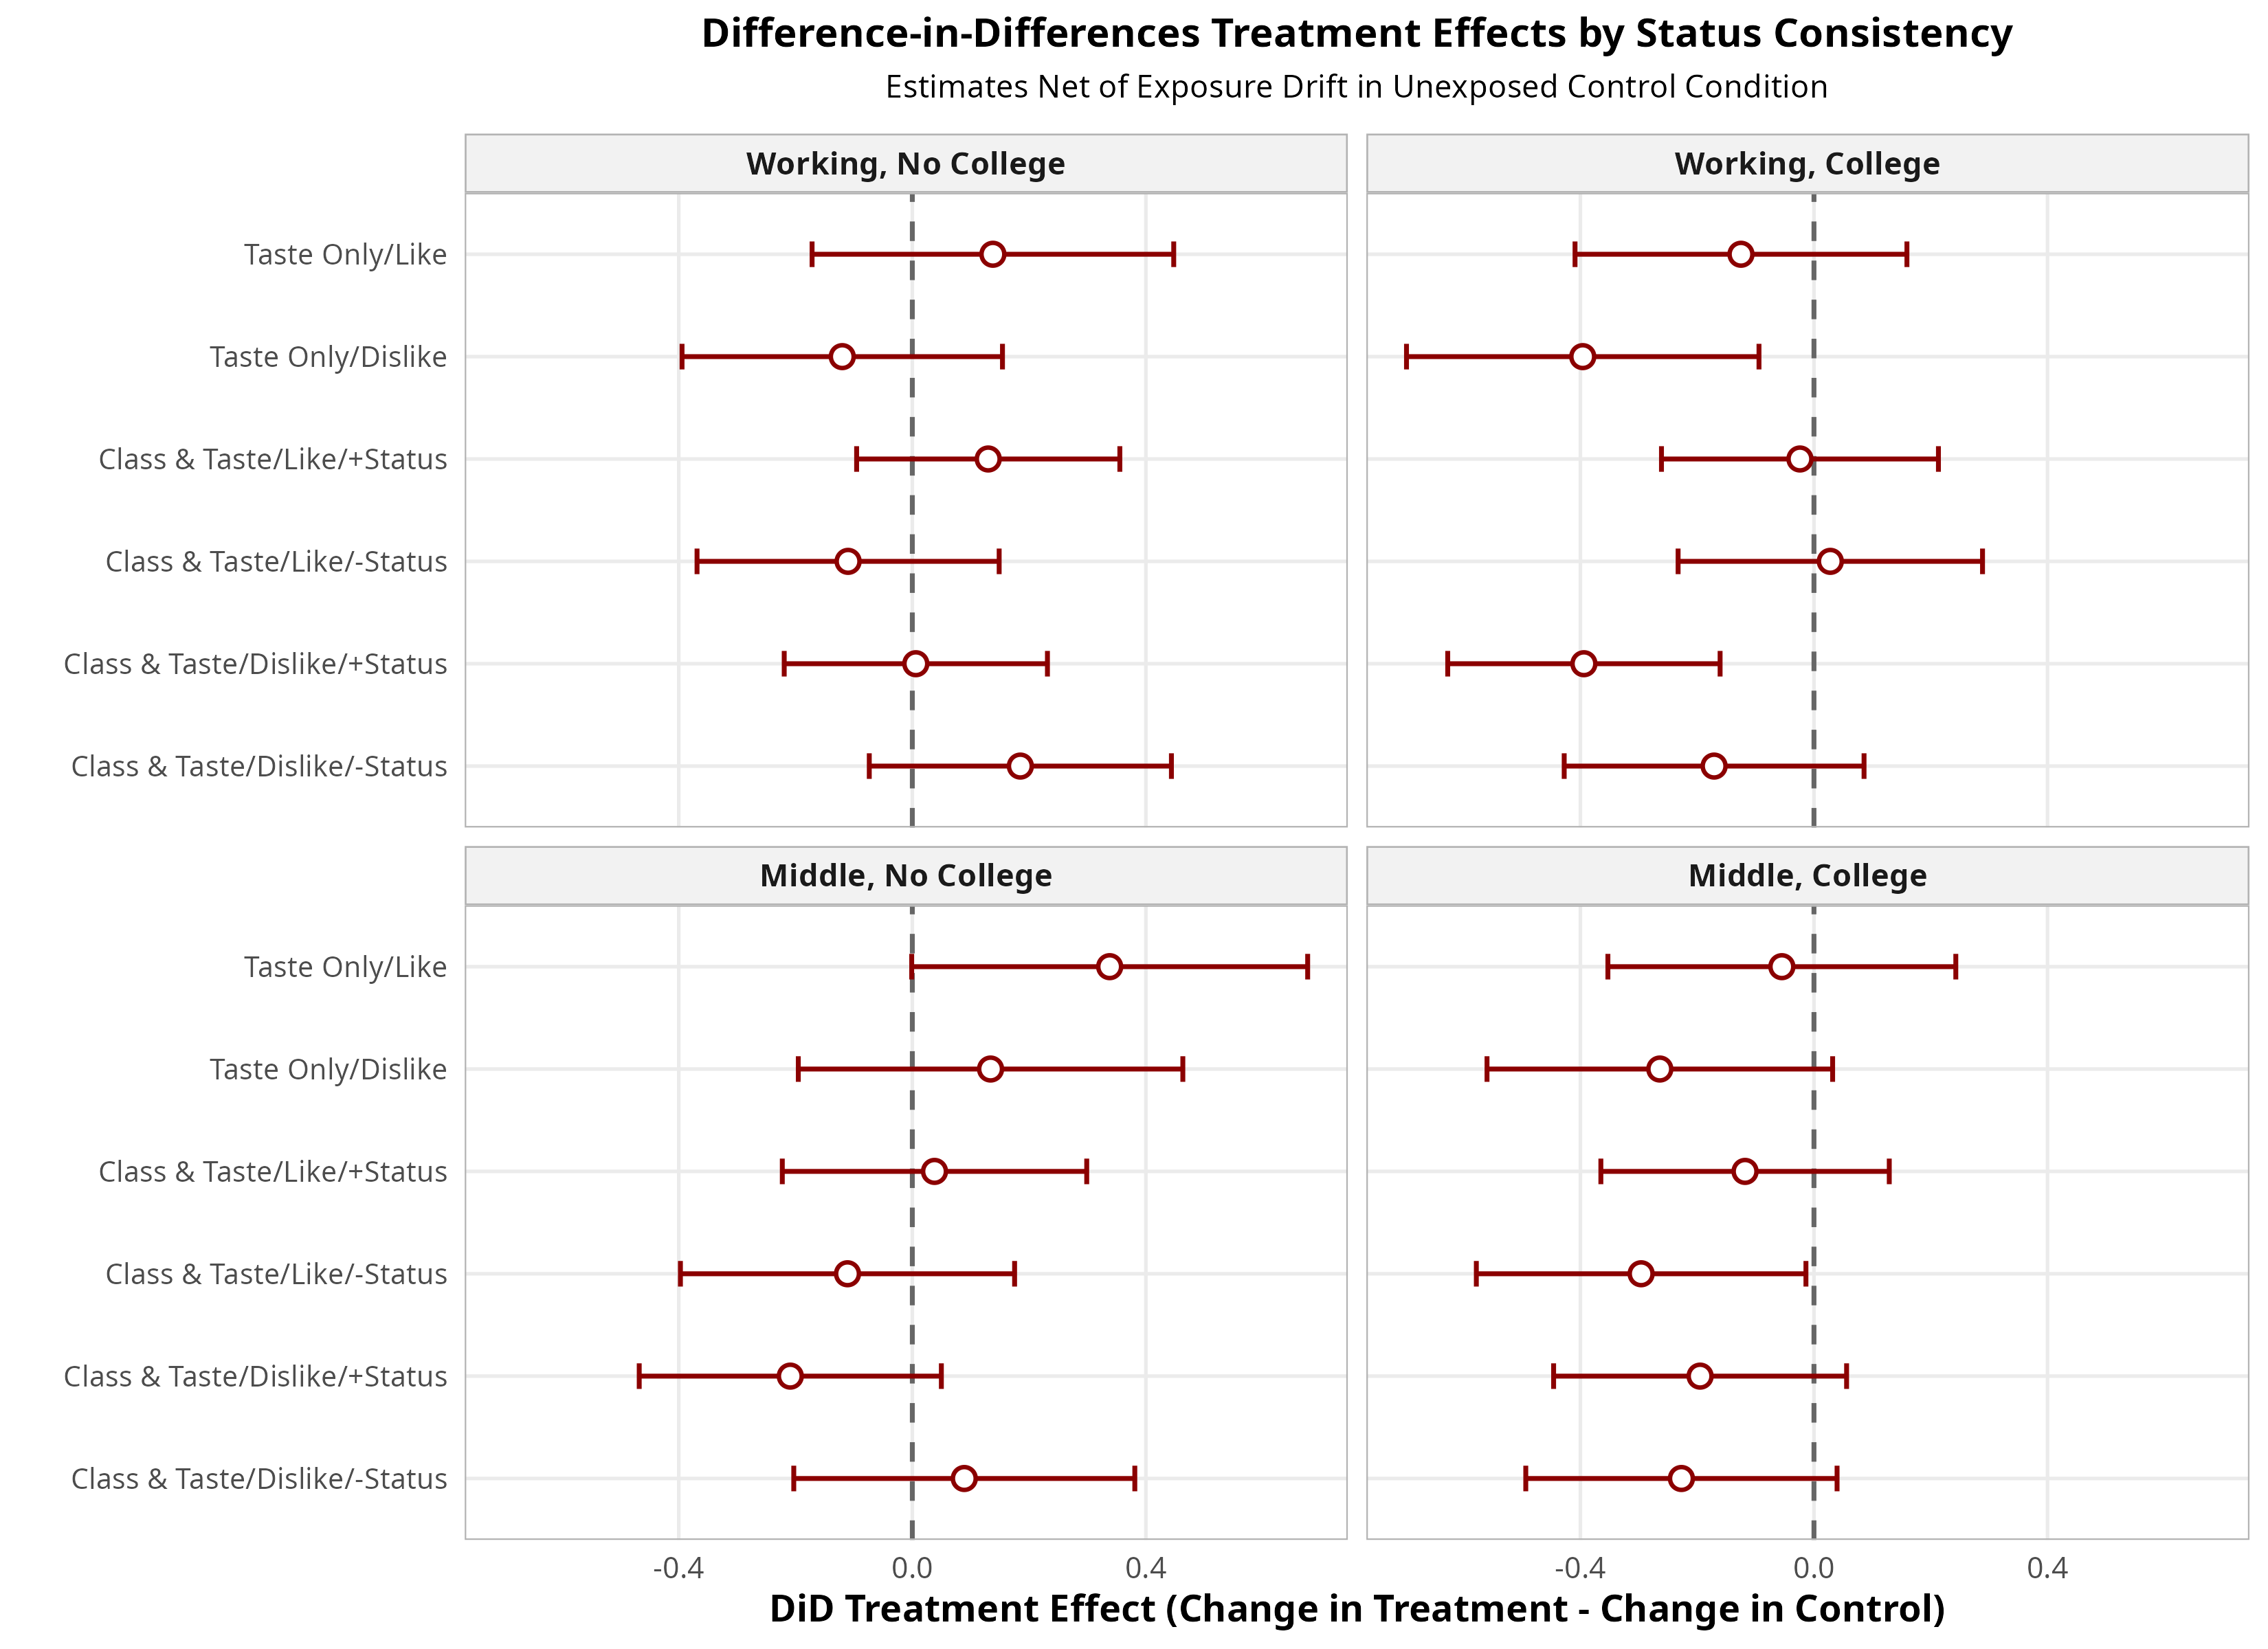
\includegraphics[width=0.95\textwidth]{figures/Figure_DiD_Forest_Status.png}
    \caption{Difference-in-Differences Treatment Effects Disaggregated by Status Consistency Group. Estimates capture condition shifts relative to the unexposed Control Condition.}
    \label{fig:did_status}
\end{figure}

Evaluating our status-differentiated hypotheses through the DiD framework yields nuanced insights across status groups. Regarding same-status alignment (\textit{Hypothesis 1}), high-status consistent respondents (Middle Class/College) align positively with high-status endorsements ($\text{raw change} = +0.28, p < 0.01$). In contrast, low-status consistent respondents (Working Class/No College) do not align with working-class peer likes ($\text{DiD} = -0.110, p = 0.404$). Instead, low-status respondents exhibit a positive shift when exposed to working-class dislikes ($\text{raw change} = +0.220; \text{DiD} = +0.185, p = 0.163$), actively reacting against the negative tastes of their own peers.

Regarding symbolic power and upward alignment (\textit{Hypothesis 2}), low-status respondents show positive movement when high-status peers like the painting ($\text{DiD} = +0.130$), reflecting cultural goodwill. However, they do not conform to high-status negative evaluations ($\text{DiD} = +0.006, p = 0.959$), once again showing valence asymmetry.

Finally, netting out counterfactual exposure drift uncovers strong support for cross-status reactance and taste abandonment (\textit{Hypothesis 3}). For high-status consistent respondents (Middle Class/College), exposure to Low-Status Likes (working-class peers endorsing the artwork) produces a statistically significant negative DiD divergence of $\text{DiD} = -0.296$ ($SE = 0.144, t = -2.06, p = 0.0391$) relative to the control condition. Because college-educated middle-class individuals naturally drift upward by $+0.200$ under mere exposure, discovering that working-class peers liked the painting actively halts and reverses their appreciation. This provides direct experimental support for Bourdieusian symbolic distinction and taste abandonment.

\subsection{Discrete Behavioral Choices: Inertia, Conformity, and Reactance}
While continuous change models identify average shifts, they mask non-linear behavioral choices. Figure \ref{fig:multinom} presents predicted probabilities from multinomial logistic regression modeling the discrete choices: Stay, Conform, and React.

\begin{figure}[ht!]
    \centering
    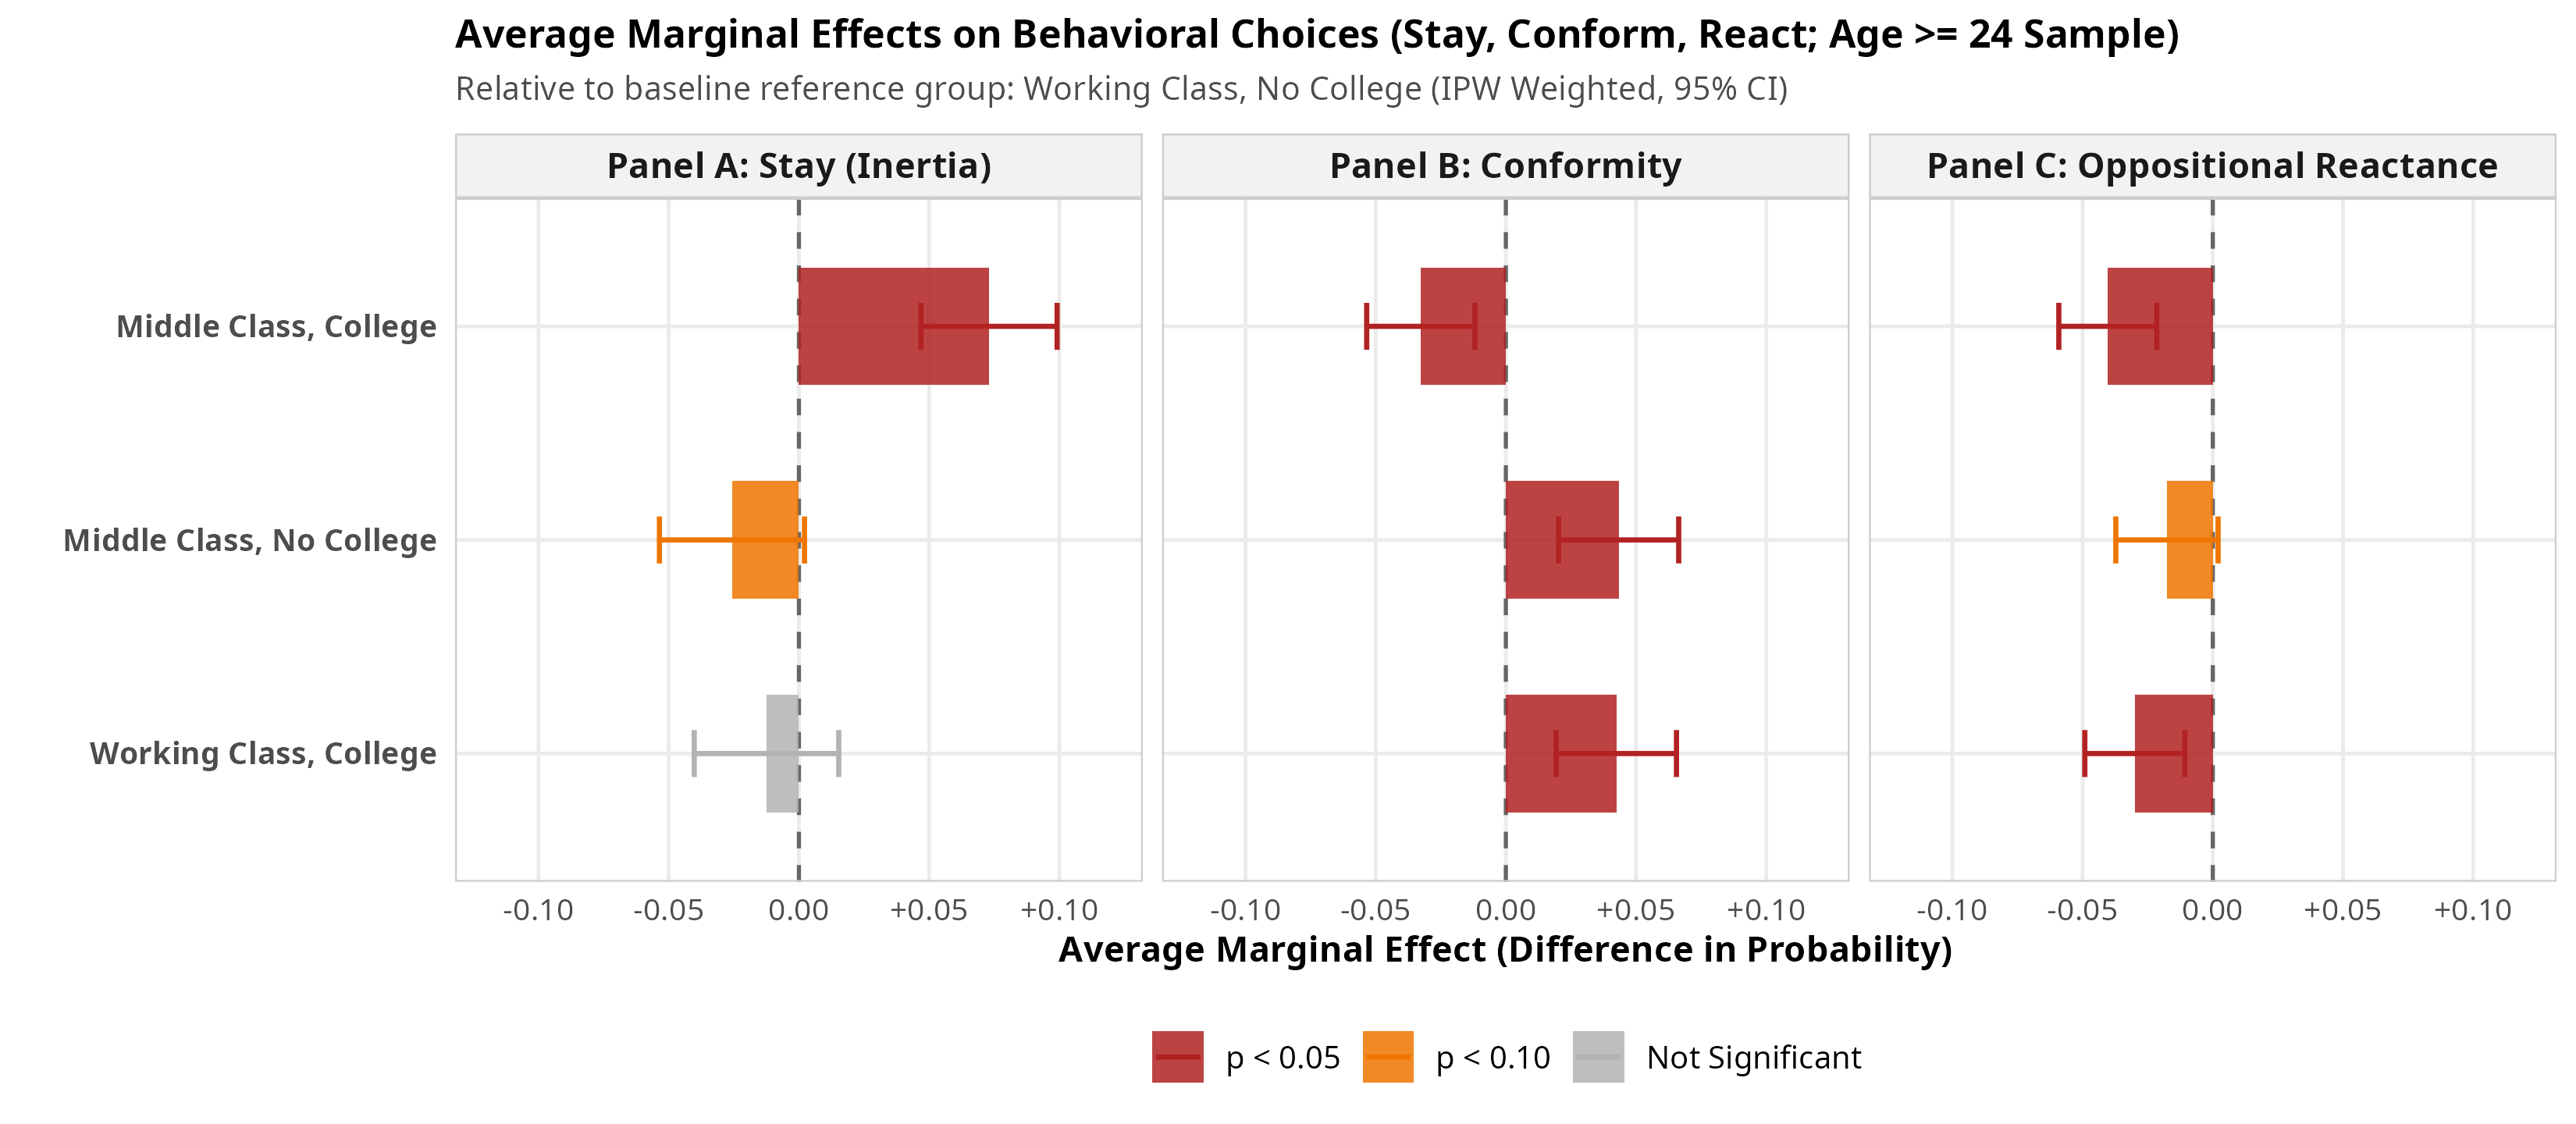
\includegraphics[width=0.85\textwidth]{figures/Figure7_MultinomialBehavior.png}
    \caption{Predicted Probabilities of Behavioral Responses (Stay, Conform, React) Across Status Groups}
    \label{fig:multinom}
\end{figure}

The behavioral model provides strong support for \textit{Hypothesis 4}. First, status consistency promotes evaluative inertia: evaluative stability (``staying'') is highest among status-consistent individuals in both high and low positions (Middle Class/College: 79.0\%; Working Class/No College: 74.4\%). Both groups occupy clear structural locations, giving them high evaluative certainty.

Second, status inconsistency produces evaluative fluidity: status-inconsistent individuals display lower inertia and higher rates of conformity (Working Class/College: 19.0\%; Middle Class/No College: 17.8\%). Third, educational capital patterns reactance: reactance is concentrated among non-college-educated individuals (12.0\%--13.3\%), who are more likely to move in the opposite direction of external social cues.

\section{Discussion}

\subsection{Summary of Key Results}
In this study, we investigated how access to peer aesthetic evaluations causally influences individual taste judgments in real time. Using a national survey experiment with a Difference-in-Differences design and inverse probability weighting, we resolved several ambiguities present in observational literature.

First, we established that repeated evaluation produces a positive exposure drift, but this drift is contingent on educational capital: college-educated individuals experience an intrinsic upward appreciation upon second exposure, whereas non-college individuals do not. Second, we established a pronounced \textit{valence asymmetry}: negative peer evaluations act as a veto that halts exposure drift across the board, whereas positive peer feedback facilitates appreciation conditionally. Third, using the DiD framework to net out counterfactual exposure drift revealed evidence for cross-status reactance: high-status respondents exposed to low-status likes showed a significant negative divergence ($\text{DiD} = -0.296, p = 0.0391$), providing experimental evidence for taste abandonment. Finally, discrete behavioral modeling showed that aesthetic stability (``staying'') is governed by structural status consistency rather than high status alone.

\subsection{Limitations and Suggestions for Future Work}
Several limitations of this study suggest directions for future research. In terms of operationalization and measurement, our experiment relied on a single cultural stimulus—Whistler's \textit{Nocturne}—selected for its high baseline variance. Future studies should examine whether social influence dynamics operate similarly across abstract, figurative, and commercial cultural forms.

Regarding threats to causal inference and contextual confounding, while our design randomized peer information, respondent status locations were observational. Although inverse probability weighting balanced observed demographic covariates, unmeasured psychological dispositions could contribute to status-group differences. Future research using laboratory status induction could provide complementary evidence.

Third, our study examined unidirectional influence from aggregate fictional peers to individuals. In everyday life, cultural influence operates bidirectionally within evolving social networks. Investigating how reciprocal feedback loops shape aesthetic consensus represents an important next step.

Fourth, regarding temporal granularity, our experiment measured short-term evaluative shifts over the course of a survey session. Longitudinal studies tracking whether experimentally induced taste shifts persist over weeks or months would help determine the durability of these social influence effects.

Finally, in terms of institutional scope conditions, our sample was recruited through a quota-matched online panel of U.S. adults. While providing greater demographic diversity than student subject pools, cross-national replications are needed to assess how national cultural institutions shape status distinction and conformity.

\subsection{Implications: Status Consistency and Evaluative Fluidity}
Our findings carry broad implications for sociological theories of taste and stratification. Classic cultural sociology has often framed aesthetic boundary work in vertical terms: high-status actors use exclusive tastes to mark distinction, while lower-status actors display cultural goodwill. Our results qualify this model by showing that cultural influence is bounded by valence asymmetry and structural consistency.

Most importantly, our analysis highlights status consistency as a neglected driver of aesthetic orientations. Status-consistent individuals—both high and low—display high evaluative stability, anchored in unambiguous structural locations. In contrast, status-inconsistent individuals experience normative cross-pressures that produce evaluative fluidity. By examining how structural consistency interacts with external social signals, cultural sociology can move beyond static homophily toward dynamic, interactional models of aesthetic judgment.

\bibliographystyle{apalike}
\bibliography{references}

\newpage
\appendix

\section{Statistical Power and Minimum Detectable Effect (MDE) Analysis}
To evaluate the statistical power of the design, we conducted an ex-post Minimum Detectable Effect (MDE) analysis. Assuming $\alpha = 0.05$ (two-tailed), power $= 0.80$, and an empirical repeated-measures test-retest correlation of $r \approx 0.70$, the design was powered to detect full sample trial shifts of Cohen's $d \ge 0.12$ ($N = 2,275$), condition-specific trial contrasts of $d \ge 0.19$ to $0.24$ across primary condition cells ($N \approx 280$--$295$), and subgroup status interaction effects of $d \ge 0.32$ to $0.38$ within specific status quadrants ($N \approx 100$--$180$).

\section{Survey Vignettes and Treatment Prompts}
\label{sec:appendix_vignettes}
Below we transcribe the verbatim wording and sequencing of the survey instrument administered in the 2012 study, based on the original Qualtrics protocol.

\subsection*{1. Baseline Measurement (Trial 1)}
Respondents were presented with the high-resolution image of James McNeill Whistler's \textit{Nocturne: Blue and Gold -- Old Battersea Bridge} (1872) and asked:
\begin{quote}
\textit{``Please look at this painting for a few seconds. Give us your first impression of this painting -- how much do you like it?''}
\end{quote}
Responses were recorded on a 7-point Likert scale: 1 = ``I like it very much'', 2 = ``I like it'', 3 = ``I like it just a little'', 4 = ``I neither like it nor dislike it'', 5 = ``I dislike it just a little'', 6 = ``I dislike it'', and 7 = ``I dislike it very much'' (plus a visual filter option ``I can't see the image''). Items were reverse-coded in data processing so that 7 indicates highest affinity and 1 indicates lowest affinity.

\subsection*{2. Experimental Treatment Vignettes}
Following their initial evaluation, respondents assigned to experimental conditions were exposed to peer feedback. Notably, the prompt did \textit{not} describe the evaluating group in relative terms to the participant; instead, it presented absolute descriptive characteristics of the alter group, allowing social proximity or distance to emerge relationally from the participant's own social location.

In the Treatment Conditions combining class status and taste information, respondents read:
\begin{quote}
\textit{``Thank you for your response. Our survey so far indicates that the group of people most likely to say that they [LIKE / DISLIKE] the painting you saw have completed\dots''}
\end{quote}
For Low Cultural Capital (LCC) peers, the description read: \textit{``\dots high school but did not go to college, and work in a food service job.''} For Economic Specialists (ES / High Cultural Capital), it read: \textit{``\dots a Bachelor's degree in Business but no additional degrees, and work at a financial investment firm.''} For Cultural Specialists (CS / High Cultural Capital), it read: \textit{``\dots several advanced degrees including a PhD, and work at a college or university.''}

Immediately following the vignette, respondents were asked: \textit{``Given only what you know about this group's education, occupation, and opinion about the painting, how similar do you think you are to the people in this group?''} (with response options: Very similar, Somewhat similar, Just a little similar, Not very similar, or Not at all similar). Treatment respondents then answered an attribution probe: \textit{``In the last question, when you thought about how similar you are to the people in this group, which factor was most influential?''} (with options: Their education and/or occupation, Their opinion about the painting, or A combination of both).

In the Taste-Only Control Condition, respondents were told: \textit{``Thank you for your response. Other people who have taken this survey recently have said that they [LIKE / DISLIKE] the painting you saw. Given only what you know about these people's opinion about the painting, how similar do you think you are to them?''} Finally, respondents in the pure No-Alter Control Condition received no feedback screen or peer cues whatsoever, proceeding directly to the intervening survey block.

\subsection*{3. Intervening Survey Battery}
Between Trial 1 and Trial 2, all respondents completed substantive survey sections comprising full educational history (highest degree attained and college major field), intergenerational educational capital (parental bachelor's degree attainment), employment status and detailed 22-category Standard Occupational Classification (SOC), annual personal pre-tax income (23 income brackets), subjective social class self-identification (Lower class, Working class, Middle class, Upper class), and an extensive musical taste battery assessing liking, listening frequency, favorite genre, and perceived audience stereotypes across 20 musical genres.

\subsection*{4. Post-Treatment Measurement (Trial 2)}
Following the intervening modules, respondents were re-shown the identical artwork and asked:
\begin{quote}
\textit{``Please look at this painting for a few seconds again. Give us your final impression of this painting -- how much do you like it?''}
\end{quote}
recorded on the identical 7-point Likert scale.

\section{Robustness Check: Alternative Definition of Social Class}
Restricting the subjective class definition strictly to respondents self-identifying as ``working class'' or ``middle class'' (excluding lower and upper class extremes) produces identical conclusions: status-consistent groups maintain the highest stay rates (Middle/College: 78.2\%; Working/No College: 74.7\%) and status-inconsistent groups maintain the highest conformity rates (Middle/No College: 17.9\%; Working/College: 16.9\%).

\end{document}
